\chapter{Praktická část}
\label{5-postup}

\section{Aktualizace pluginu do verze 1.0}
Po dokončení pluginu \textit{GTFS Loader} v předmětu Free Software GIS měl plugin veškerou základní
funkcionalitu, kterou měl mít (odkaz na plugin \href{https://github.com/ctu-fgis/2020-b-qgis-gtfs-plugin}
{\underline{zde}}). 
Tou bylo načítání GTFS ZIP souboru do systému QGIS,
rozbalení ZIP souboru, načtení \zk{CSV} souborů do geodatabázového formátu GeoPackage (dále \zk{GPKG}),
vytvoření vektorových vrstev pro soubory \textit{stops.txt} a \textit{shapes.txt},
symbologie vektorové vrstvy \textit{shapes} a vložení \zk{CSV}  souborů a vrstev do projektu QGIS.

\begin{figure}[H] \centering
    
\includegraphics[width=100pt]{./pictures/logo-plugin.png}
    \caption[Logo pluginu GTFS Loader]{Logo pluginu GTFS Loader}
	\label{fig:logo-plugin}              
\end{figure}   

%% ML: pridejte screenshot celeho pluginu/QGISu (nikde se neobjevuje) MK: v dodatku

Plugin obsahoval nedostatky, které bylo nutné před zveřejněním v QGIS repo\-zitáři vyřešit. 
Proto byl veškerý proces přesunut na pozadí, aby celý QGIS software \uv{nezamrzal} a
mohly se při jeho výpočtech provádět i jiné akce. To se provedlo díky třídě programovacího jazyka Python \textit{QgsTask}
a jejím metodám, které byly zděděny z této třídy. \cite{QgsTask}

Pro zobrazování procesu během výpočtu byla použita třída \textit{QProgressBar} a její metody.
Zobrazení postupu bylo implementováno do lišty zpráv systému QGIS spolu s chybovými hláškami.

\begin{figure}[H] \centering
    
\includegraphics[width=400pt]{./pictures/loading.png}
    \caption[Ukazatel průběhu (ProgressBar) v liště systému QGIS]{Ukazatel průběhu (ProgressBar) v liště systému QGIS}
	\label{fig:ProgressBar v liště systému QGIS}              
\end{figure}     

\section{Tvorba vizualizace tarifních pásem (experimentální verze pluginu 2.0)}

V následujících podkapitolách je uveden postup tvorby rozšíření pluginu.
Nejprve bylo vytvořeno dialogové okno pro potvrzení nebo odmítnutí tvorby tarifních pásem (podkapitola \ref{dialog}).
Dále byl vytvořen hrubý tvar tarifních pásem z rozdílným po\-stupem pro tarifní pásma P, 0 a B
a pro tarifní pásma 1 až 9 (podkapitola \ref{hruby_tvar}). 
Tarifní pásma 1 až 9 byla tvořena se vzájemně oddělenými vektorovými vrstami.
Hrubý tvar nebyl vizuálně vzhledný a k referenčním tarifním pásmům
z portálu \textit{Opendata hlávního města Prahy} se nepřibližoval, takže byl zjemněn (podkapitola \ref{vyhlazeni}).
Zároveň byla zjemněna i hraniční pásma, což byla nově vytvořená tarifní pásma pro zastávky
na hranici mezi pásmy, které se nepodařilo spojit (podkapitola \ref{hranice}). 
Hladká tarifní pásma byla následně spojena do jedné vektorové vrstvy (podkapitola \ref{seskupeni}) a 
byla k ní přidána symbologie (podkapitola \ref{symbologie}).

Při průzkumu technologií byla možnost vypracovat tvorbu tarifních pásem pomocí Grafického modeláře,
který je zabudovaný v systému QGIS.
Kvůli omezeným možnostem úprav nástrojů se z těchto myšlenek upustilo a byl vytvářen postup
do~prázdného skriptu v programovacím jazyce Python pomocí nástrojů systému QGIS.

Pro použití nástrojů sysému QGIS ve skriptu programovacího jazyka Python bylo potřeba importovat modul \textit{processing},
který má funkci \textit{run}, do které se vkládají dva parametry. První parametr je ID nástroje
ve formě \textit{řetězce} a druhý je \textit{slovník} vstupních parametrů. Vstupní parametry se lze dozvědět
z QGIS dokumentace. \cite{QGIS_docs}

\subsection{Dialogové okno pro tvorbu tarifních pásem}
\label{dialog}

Aby se uživatel při používání pluginu mohl rozhodnout, či chce vytvářet tarifní pásma nebo ne, bylo vytvořeno
dialogové okno pomocí PyQt (viz obrázek \ref{fig:dialog}). Toto dialogové okno se vždy zobrazí po stisknutí tlačítka
\textit{Load} pro načtení GTFS ZIP souboru. Jak je v závorce napsáno, tvorba tarifních pásem je zatím jen pro GTFS
dataset PID\_GTFS. Tvorba tarifních pásem pro ostatní GTFS soubory může být jako námět pro další závěrečné práce nebo ho mohou 
vypracovat uživatelé služby GitHub.

\begin{figure}[H] \centering
    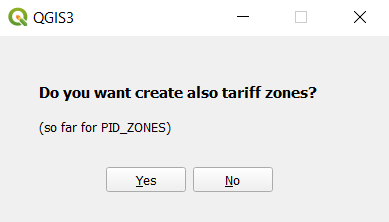
\includegraphics[width=180pt]{./pictures/dialog.png}
    \caption[Dialogové okno s možností tvořit/netvořit tarifní pásma]{Dialogové okno s možností tvořit/netvořit tarifní pásma}
	\label{fig:dialog}                                
\end{figure}

Ovládání dialogového okna je jednoduché. Disponuje běžnými tlačítky pro mi\-nimalizaci okna a vypnutí okna, což mimochodem
zruší kompletně proces načítání GTFS souboru. Mimo to tu jsou dvě tlačítka Yes/No, které buďto povolí vytváření tarifních
pásem anebo nepovolí a proces běží jako ve verzi pluginu 1.0.

Kvůli přehlednosti byl založen nový skript \textit{zones.py} v programovacím jazyce Python se třídou \textit{GtfsZones}. 
Instance této třídy byla vytvořena v hlavním skriptu \textit{GTFS.py}.

\subsection{Hrubý tvar tarifních pásem}
\label{hruby_tvar}

GTFS dataset obsahuje povinný \zk{CSV} soubor \textit{stops.txt} (viz kapitola \ref{stops.txt}). Tento soubor obsahuje mimo
jiných polí také pole \textit{zone\_id}, které bylo klíčové při tvorbě tarifních pásem.
Pole \textit{zone\_id} má datový typ \textit{řetězec} a znamená, ve kterém ta\-rifním
pásmu daná zastávka leží. Verze 1.0 pluginu \textit{GTFS Loader} soubor \textit{stops.txt} převádí do~vektorové vrstvy
ve formě bodů. Z této bodové vrstvy byla vytvořena vektorová vrstva Voronoi 
diagramů nástrojem \textit{Voronoi polygons} v programu QGIS. 

Vstupem do tohoto nástroje byla vektorová vrstva stops a výstupem byly Voronoi polygony.

\begin{figure}[H] \centering
    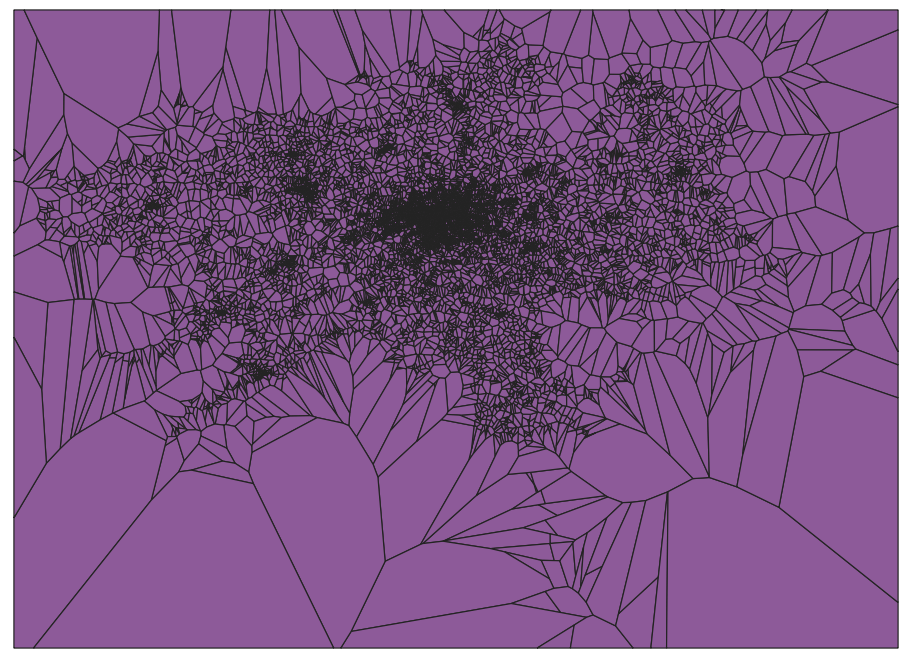
\includegraphics[width=400pt]{./pictures/voronoi-stops.png}
    \caption[Voronoi polygony pro všechny zastávky]{Voronoi polygony pro všechny zastávky}
	\label{fig:voronoi-stops}              
\end{figure}
  
Pro každé tarifní pásmo byly vybrány zastávky pomocí třídy \textit{QgsVectorLayer}
a její metody \textit{selectByExpression}, která má parametr \textit{expression} ve formě datového
typu \textit{string}. 
Třída \textit{QgsVectorLayer} zároveň vrací vektorovou vrstvu, která může být považována jako vstup do nástroje QGIS.

\subsubsection{Tarifní pásma P, 0 a B}

Speciálně pro tarifní pásma na území Prahy (tarifní pásma P, 0 a B) byl tvořen rozdílný postup
než pro ostatní pásma ležící ve Středočeském kraji a okolí. Do~meto\-dy \textit{selectByExpression} byl vložen
parametr s dotazem: 

\["zone\_id"\ IN\ ('P','0','B')\ AND\ "location\_type" = 0\]

Po proběhnutí tohoto dotazu byly vybrány všechny zastávky ležící v tarifních pásmech P, 0 a B. 

V zadávaném výrazu figuruje taktéž údaj o poli \textit{location\_type}, což je typ lokace. 
Hodnota nuly (nebo prázdná hodnota) je právě lokace zastávky viz \ref{stops.txt}.

Některé zastávky se nacházely na stejném místě a měly duplicitní geometrii, což~vytvářelo v dalším
zpracování problém s duplicitními polygony. Aby se takové věci ve~výsledku zamezilo, byl použit nástroj   
\textit{Delete duplicate geometries}, který~ve~vstupní vektorové vrstvě nalezne duplicitní geometrie a smaže je.

\begin{figure}[H] \centering
    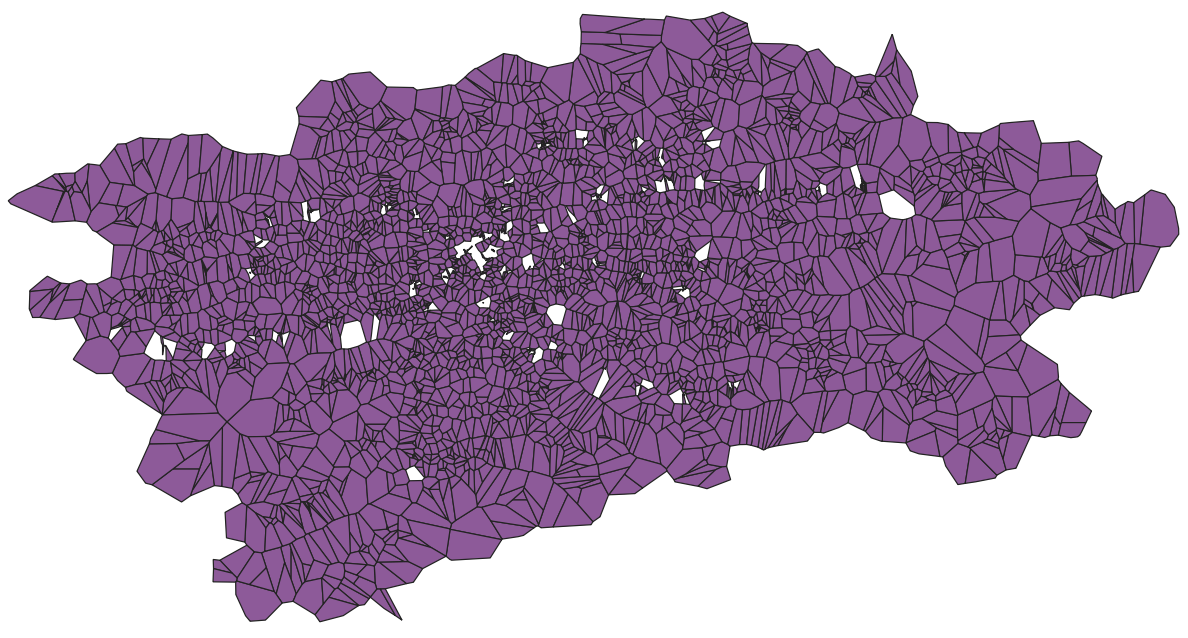
\includegraphics[width=400pt]{./pictures/voronoi-selected-P0B.png}
    \caption[Vybrané Voronoi polygony pro tarifní pásma P, 0 a B]{Vybrané Voronoi polygony pro tarifní pásma P, 0 a B}
	\label{fig:voronoi-selected}              
\end{figure}

Pro vybrané zastávky bylo potřeba vybrat ty Voronoi polygony, které svou
pozicí dané zastávky protínaly. To bylo provedeno nástrojem \textit{Select by location},
do kterého vstupovala vrstva vybraných zastávek a vrstva Voronoi polygonů. Výsledkem tohoto nástroje byla
vektorová vrstva vybraných Voronoi polygonů. Jako příklad v obrázku zde budu uvádět tarifní pásmo 2.
% zde upravit obrázky, bude změněno pro tarifní pásmo P,0,B

Tyto polygony byly následně nástrojem \textit{Dissolve} spojeny do jednoho společného polygonu.
Vstupem tohoto nástroje byl výstup nástroje \textit{Select by location} a výstupem byl polygon
s jednou geometrií. 

\begin{figure}[H] \centering
    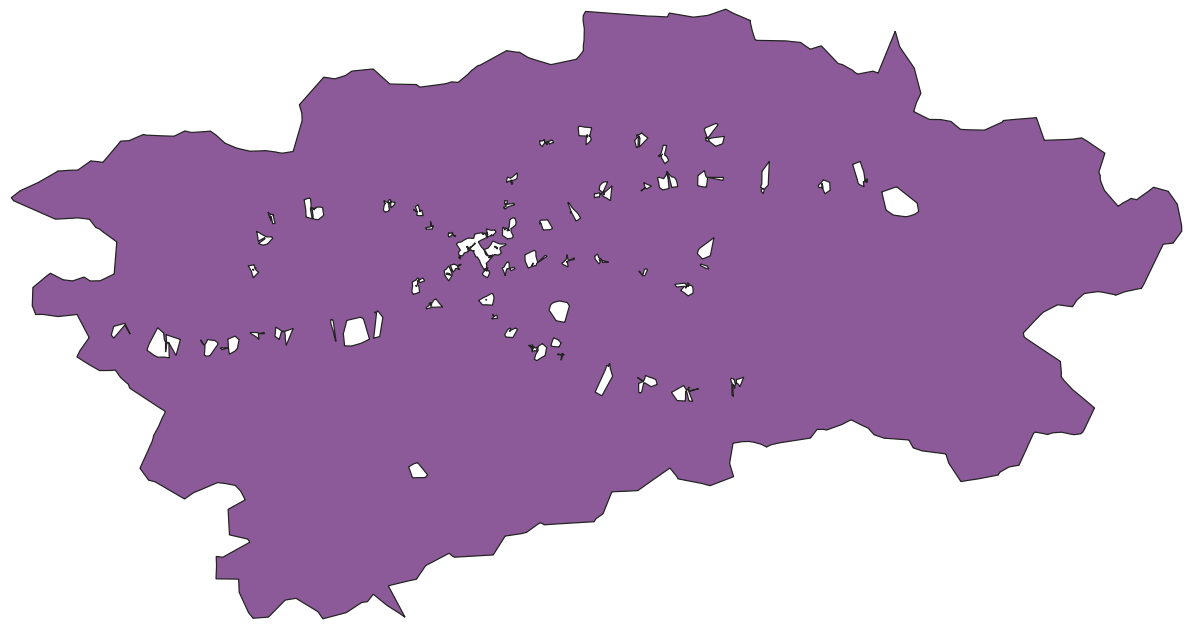
\includegraphics[width=400pt]{./pictures/dissolve-P0B.png}
    \caption[Výsledek nástroje Dissolve pro tarifní pásma P, 0 a B]{Výsledek nástroje Dissolve pro tarifní pásma P, 0 a B}
	\label{fig:dissolve}              
\end{figure} 

Kvůli mnoha zastávkám, které v oblasti pásem P, 0 a B v poli \textit{zone\_id} obsahovaly hodnotu \textit{NULL},
vznikla uvnitř polygonu spousta děr. V těchto dírách někdy ležely i části malých polygonů, které 
už po nástroji \textit{Dissolve} tvořili jeden celistvý polygon. A proto nebylo možné rovnou použít nástroj Delete holes,
nýbrž nejprve nástroj \textit{Multipart to singleparts}.

Nástroj \textit{Multipart to singleparts} rozdělil jeden vícedílný polygon na jednotlivé menší polygony. Vstupem do tohoto
nástroje byl vektorová vrstva výstupu nástroje Dissolve a výstupem byl vektorová vrstva s rozděleným polygonem.

Poté se pomocí metody \textit{selectByExpression} třídy \textit{QgsVectorLayer} vyhledal nej\-větší polygon.
Výraz vkládaný jako parametr do metody \textit{selectByExpression} byl následující:

\[\$area = maximum(\$area, "zone\_id")\]

Takový polygon byl uložen do nové vektorové vrstvy. 

\begin{figure}[H] \centering
    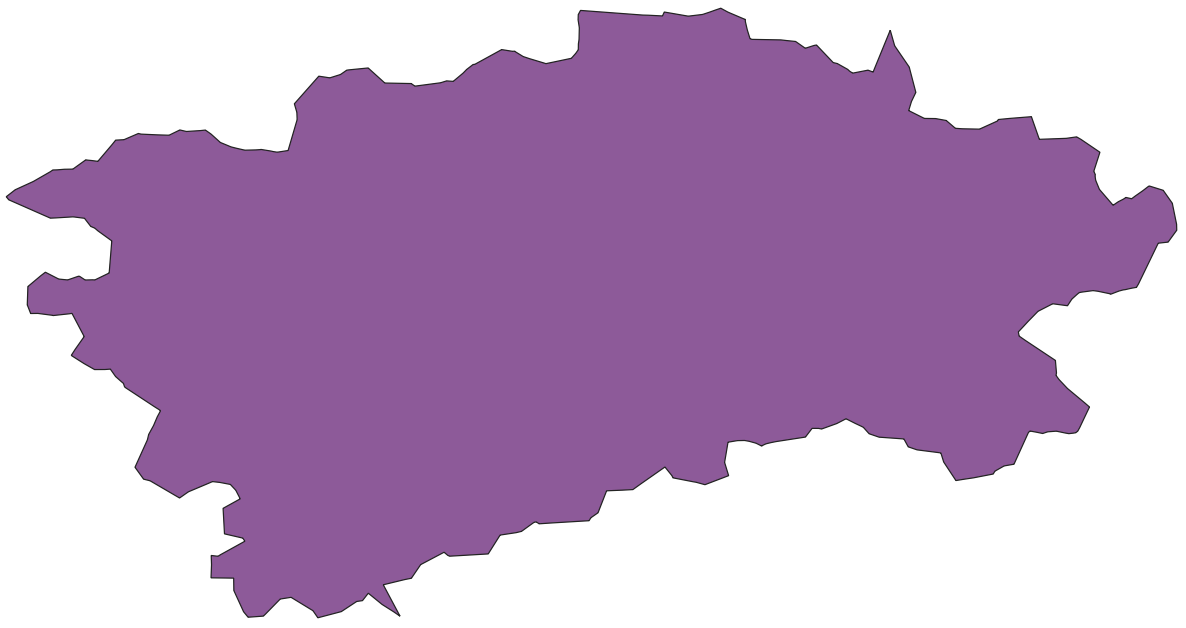
\includegraphics[width=400pt]{./pictures/without-holes-P0B.png}
    \caption[Výsledek nástroje Delete holes pro tarifní pásma P, 0 a B]{Výsledek nástroje Delete holes pro tarifní pásma P, 0 a B}
	\label{fig:without-holes-P0B}              
\end{figure} 

Poté již byl použit nástroj \textit{Delete holes}, který zaplnil vytvořené díry. Vstupem do tohoto nástroje byla vektorová
vrstva s největší polygonu z nástroje \textit{Dissolve}. Nástroj obsahoval volitelný parametr rozlohy, který byl
nastaven na hodnotu 500 a~se kterým se nástroj \textit{Delete holes} řídí a zaplňuje menší díry, než byl tento parametr.  

Znázornění tohoto postupu je zobrazeno zde v obrázku \ref{fig:postup-voronoi-P0B}. Toto zobrazení bylo provedeno v Grafickém modeláři.

\begin{figure}[H] \centering
    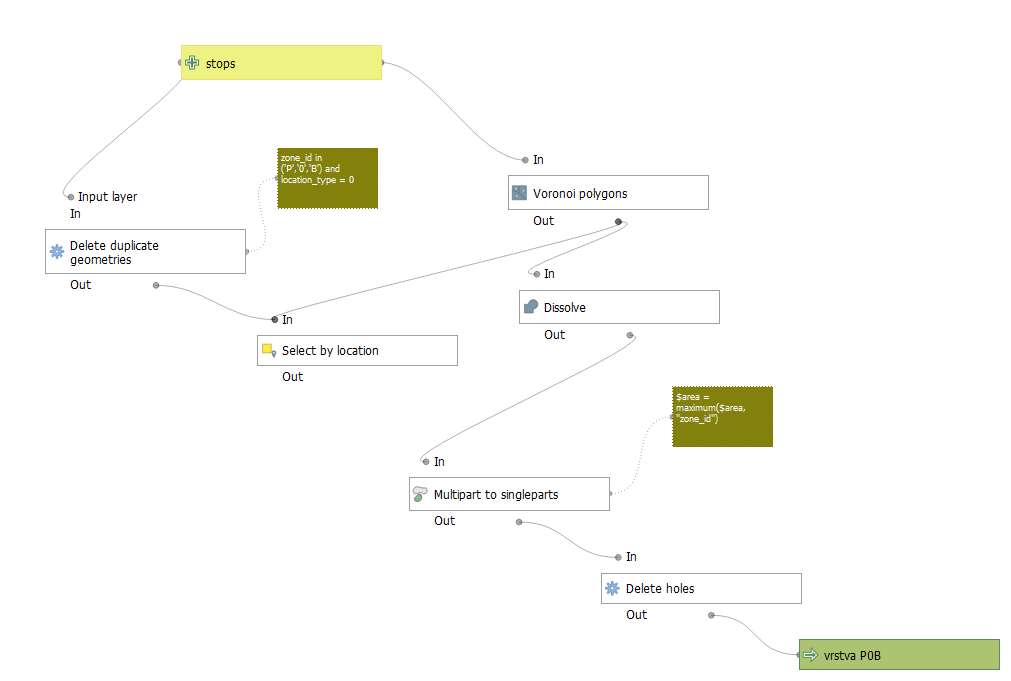
\includegraphics[width=400pt]{./pictures/postup-voronoi-P0B.png}
    \caption[Postup pro tarifní pásma P, 0 a B]{Postup pro tarifní pásma P, 0 a B}
	\label{fig:postup-voronoi-P0B}              
\end{figure}

\subsubsection{Tarifní pásma 1 až 9}
\label{tp_1az9}

Obdobný postup jako u tarifních pásem P, 0 a B, avšak znatelně jednodušší, byl proveden za pomocí
for cyklu pro tarifní pásma 1 až 9. 

Opět ty zastávky, které ležely v určitém pásmu, byly vyhledány pomocí metody \textit{selectByExpression} třídy 
\textit{QgsVectorLayer}. Pro zastávky tarifních pásem 1 až 6 to~bylo provedeno pomocí dotazu:

\["zone\_id"\ <=\ "ID\: pasma"\ AND\ "zone\_id"\ !=\ '-'\ AND\ "location\_type" = 0\]  

Pro zastávky tarifních pásem 7 až 9 pomocí dotazu:
\["zone\_id"\ =\ "ID\: pasma"\ AND\ "location\_type" = 0\] 

V dotazu pro tarifní pásma 1 až 6 byly vybrány ty zastávky, které mají hodnotu pole \textit{zone\_id} menší jak aktuální hodnota,
hodnota pole \textit{zone\_id} se nerovná \uv{pomlčce} (jelikož zastávky s touto hodnotou jsou mimo tarifní pásma)
a hodnota pole \textit{location\_type} byla rovna nule. V dotazu pro tarifní pásma 7 až 9 byly vybrány ty zastávky,
které mají hodnotu pole \textit{zone\_id} aktuální hodnotě a hodnota pole \textit{location\_type} byla rovna nule.

Důvodem pro dělení těchto dotazů byla jednak časová náročnost délky průběhu následujícího nástroje \textit{Select by location}, 
kde kvůli operátoru "<=" u dotazu pro~zastávky tarifních pásem 1 až 6 do nástroje vstupují všechny zastávky, 
které jsou hodnotou \zk{ID} menší jak aktuální hodnota. Tím se pro každé tarifní pásmo násobně zvětšuje počet zastávek,
které vstupují do nástroje \textit{Select by location}.

Pro tarifní pásma 7 až 9 byla časová náročnost stejná, jako u tarifních pásem P, 0 a B.

Hlavním důvodem avšak bylo \uv{zalepení} děr, které vznikaly u vyhlazení tvaru tarifních pásem v kapitole \ref{vyhlazeni}.  

Následně byl pouze spuštěn \textit{Dissolve} pro spojení Voronoi polygonů, což bylo vstupem do tohoto nástroje,
do jednoho celistvého polygonu, což bylo výstupem tohoto nástroje.

V následujícím obrázku \ref{fig:postup-voronoi-1az9} je souhrnně zobrazen postup tarifní pásma 1 až 9.

\begin{figure}[H] \centering
    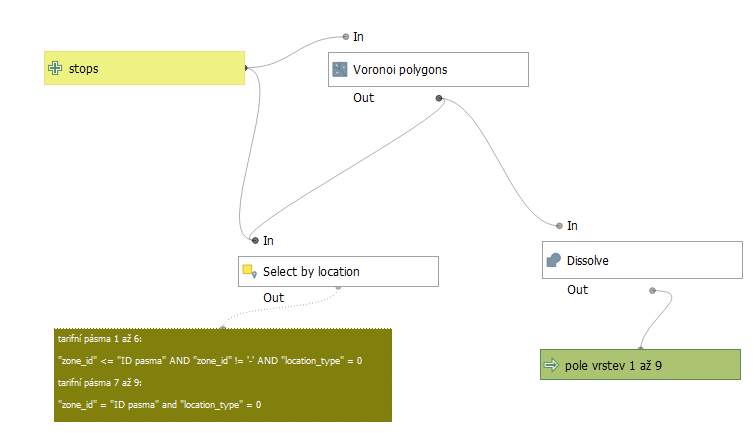
\includegraphics[width=400pt]{./pictures/postup-voronoi-1az9.png}
    \caption[Postup pro tarifní pásma 1 až 9]{Postup pro tarifní pásma 1 až 9}
	\label{fig:postup-voronoi-1az9}              
\end{figure}

\subsection{Vyhlazení tvaru tarifních pásem}
\label{vyhlazeni}

Pro vytvoření kartograficky přesných a vizuálně přijatelnějších tarifních pásem dosa\-vadní postup nestačil.
V souboru \textit{stops.txt} datasetu PID\_GTFS existovaly takové zastávky, které měly tarifní pásmo sdílené
na rozhraní pásem. Těmito zastávkami měla podle pravidel organizace ROPID tarifní pásma procházet.

Bylo nutné navrhnout další průběh úpravy dosavadního tvaru tarifních pásem, který takovou podmínku zahrnuje
a zároveň vyhlazuje tvar polygonů pro lepší vizuální tvar.  

Ze spojených polygonů byla vygenerována vektorová vrstva bodů nástrojem
\textit{Extract vertices}, která představovala vrcholy spojených polygonů. Pro tuto vrstvu
bylo vstupem výstup nástroje \textit{Dissolve} a výstupem byl vektorová vrstva bodů 
doplněná o pole (mimo původních polí z vektorové vrstvy \textit{stops}) jako \textit{vertex\_index,
vertex\_part, vertex\_part\_ring, distance} a \textit{angle}.
Hodnoty těchto polí avšak nebyly využity v dalším výpočtu.

\begin{figure}[H] \centering
    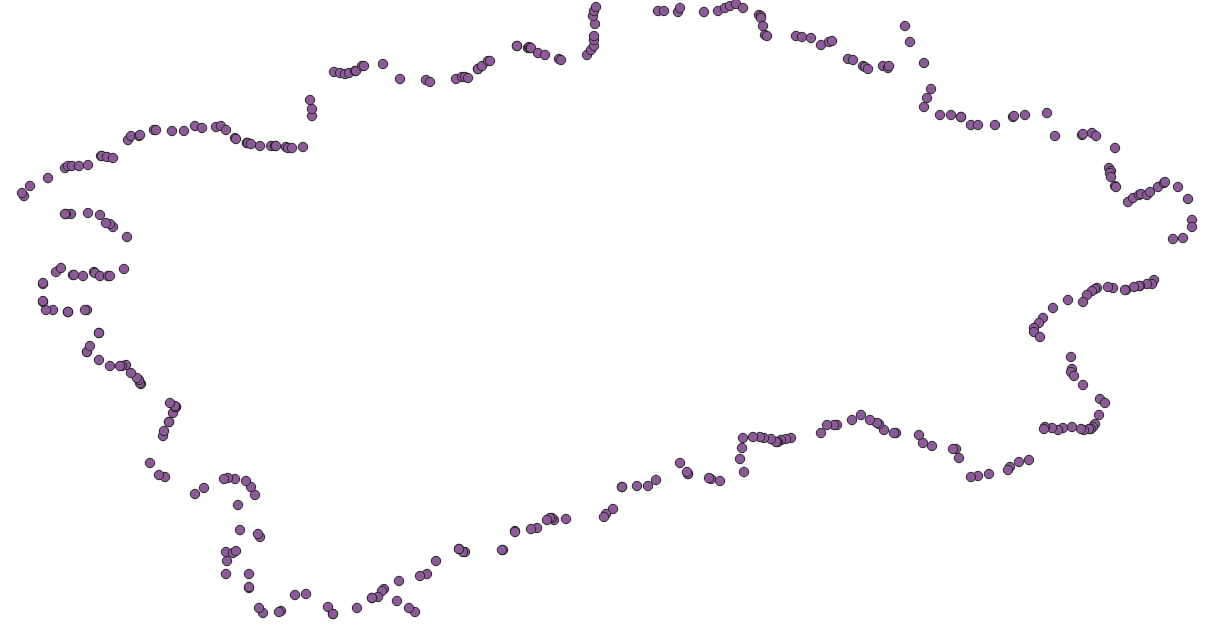
\includegraphics[width=400pt]{./pictures/vertices-P0B.png}
    \caption[Výsledek nástroje Extract vertices]{Výsledek nástroje Extract vertices}
	\label{fig:vertices-P0B}              
\end{figure} 

Dále byly s pomocí třídy \textit{QgsVectorLayer} a její metody \textit{selectByExpression} vybrány 
z původní vektorové vrstvy \textit{stops} ty zastávky, které ležely na hranici tarifních pásem.
Takové zastávky obsahovaly v poli \textit{zone\_id} hodnoty tarifních pásem od\-dělené čárkami.
Například pro zastávky mezi pásmem 1 a 2 byla hodnota pole \textit{zone\_id} uvedena jako \uv{1,2}.

Pro tarifní pásma P, 0 a B byl použit dotaz:

\["zone\_id"\ NOT\ IN\ ('P',\ '0',\ 'B',\ '1',\ '2',\ '3',\ '4',\ '5',\ '6',\ '7',\ '8',\ '9')\]
\[AND\ ("zone\_id"\ LIKE\ '\%P\%'\ OR\ "zone\_id"\ LIKE\ '\%0\%'\]
\[OR\ "zone\_id"\ LIKE\ '\%B\%')\]

Pro tarifní pásma 1 až 9 byl použit dotaz:
\["zone\_id"\ LIKE\ "ID\: pasma\ i,ID\: pasma\ i+1"\]

Vybraná tarifní pásma byla uložena do nové vektorové vrstvy pro následné a~pozdější použití viz kapitola \ref{hranice}.

Následně pro každé tarifní pásmo nástrojem \textit{Merge vector layers} byly spojeny tři vektorové vrstvy: hraniční zastávky, 
zastávky uvnitř tarifního pásma a body z~výstupu nástroje \textit{Extract vertices}.
Tyto zmiňované vektorové vrstvy byly vstupem do tohoto nástroje a výstupem byla 
vektorová vrstva spojených bodů. 

\begin{figure}[H] \centering
    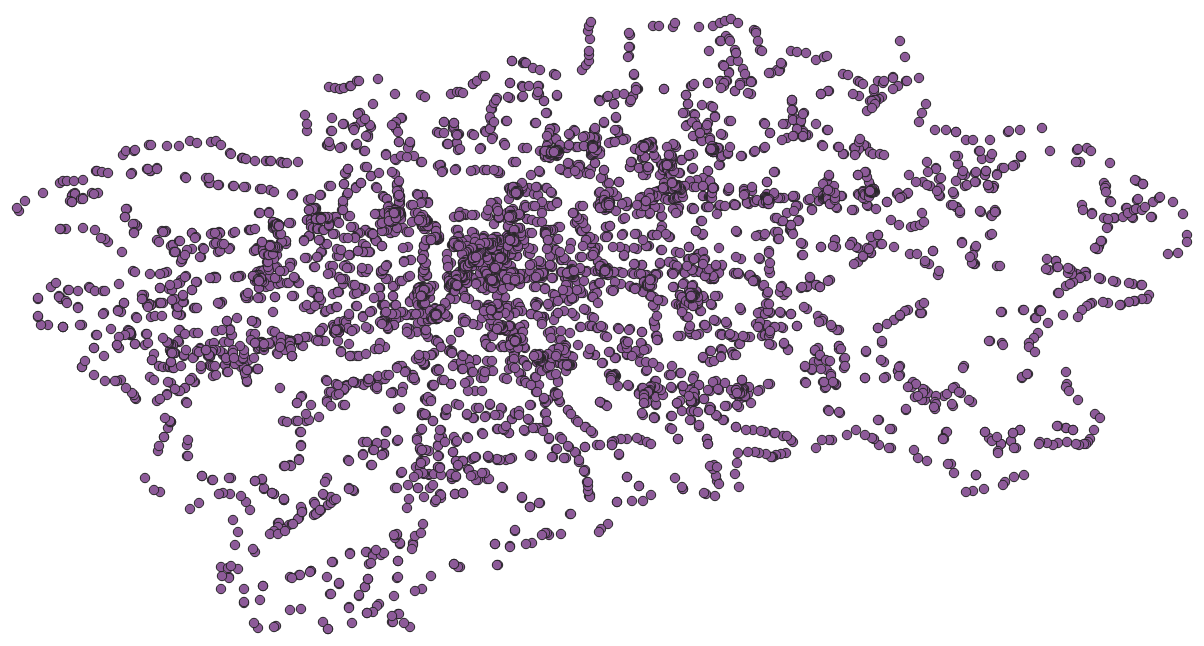
\includegraphics[width=400pt]{./pictures/merged-P0B.png}
    \caption[Spojené body třech vektorových vrstev pomocí nástroje Merge vector layers]{Spojené body třech vektorových vrstev pomocí nástroje Merge vector layers}
	\label{fig:merged-P0B}              
\end{figure} 

Pro spojení bodů a vytvoření jakési obálky byl nejdříve vyzkoušen nástroj \textit{Mi\-nimum bounding box} s možností Convex Hull,
což je aplikace algoritmu Konvexní obálky viz kapitola \ref{konv_obalka}. Tento způsob však velmi zjednodušoval tvar
tarifních pásem, a~proto~nástroj \textit{Minimum bounding box} nebyl použit.

Byla zvolena další možnost nástroje systému QGIS spojující body do jisté obálky. Tím nástrojem byl \textit{Concave hull (alpha shapes)} 
využívající aproximaci alpha-shapes viz kapitola \ref{konk_obalka}.

Vstupem nástroje tedy byla vrstva spojených bodů, což byl první parametr
nástroje. Dalším parametrem byl práh (Threshold) s datovým typem \textit{čísla}, který byl volen od 0 do 1,
kdy 0 znamenala maximum konkávní obálky a 1 konvexní obálky. Po několika testovacích spuštění byla 
určena hodnota 0,09 jako nejlepší hodnotou pro tvorbu tarifních pásem. Dalším parametrem bylo Povolení děr (Allow holes) 
s~datovým typem \textit{boolean}, který byl nastaven na \textit{False}.
Posledním parametrem bylo Rozdělit vícedílnou geometrii na jednotlivé části (Split multipart geometry 
into singlepart geometries) taktéž s datovým typem \textit{boolean}, který byl nastaven na \textit{True}.  
Výstupem byla polygonová vrstva konkávní obálky. 

Vytváření konkávní obálky bylo dalším důvodem pro dělení atributových dotazů v kapitole \ref{tp_1az9} pro 
zaplnění děr v tarifních pásmech 6 a nižších.  

\begin{figure}[H] \centering
    
\includegraphics[width=400pt]{./pictures/concaveHull-P0B.png}
    \caption[Konkávní obálka]{Konkávní obálka}
	\label{fig:concaveHull-P0B}              
\end{figure} 

Z konkávní obálky byla pomocí nástroje Simplify \uv{zjednodušena} geometrie polygonové vrstvy. Tento nástroj
využívá tři druhy zjednodušení vektorové vrstvy: založené na vzdálenosti (algoritmus \uv{Douglas-Peucker}),
založené na ploše (algoritmus \uv{Visvalingam}) a přichytávání geometrií k mřížce.

Pro můj postup byl zvolen první volba zjednodušení, pomocí algoritmu \uv{Douglas-Peucker} viz kapitola \ref{generalizace_zjemneni}.


Do nástroje \textit{Simplify} byl vstupem výsledek nástroje \textit{Concave hull (alpha shapes)}, parametrem byl výběr algoritmu 
a nastavení hodnoty tolerance vzdálenosti. Výstupem byla polygonová vektorová vrstva.

\begin{figure}[H] \centering
    
\includegraphics[width=400pt]{./pictures/simplify-P0B.png}
    \caption[Výsledek nástroje Simplify]{Výsledek nástroje Simplify}
	\label{fig:simplify-P0B}                                
\end{figure}

Výstup nástroje \textit{Simplify} byl vstupem do nástroje \textit{Smooth}. Tento nástroj vy\-hlazuje geometrie
liniové nebo polygonové vrstvy pomocí Chaikinova algoritmu viz~ka\-pitola \ref{vyhlazeni}.

\begin{figure}[H] \centering
    
\includegraphics[width=400pt]{./pictures/smooth-P0B.png}
    \caption[Výsledek nástroje Smooth]{Výsledek nástroje Smooth}
	\label{fig:smooth-P0B}                                
\end{figure}

U nástroje \textit{Smooth} byly zvoleny tři parametry - počet iterací, offset a maximální úhel.
Počet iterací znamená, kolik vyhlazovacích iterací bude použito pro každou geometrii.
Hodnota počtu iterací byla nastavena na 10, což byla maximální volitelná hodnota (pro co největší hladkost).
Parametr offset znamená, jak \uv{těsně} vyhlazené geometrie sledují původní geometrie.
Zde byla ponechána výchozí hodnota 0,25. A~poslední parametr maximálního úhlu lze použít
k zabránění vyhlazení uzlů s~velkými úhly. Zde byla také ponechána výchozí hodnota 180°.
Výstupem nástroje byla polygonová vektorová vrstva.

Níže je souhrnně zobrazen postup této části pomocí Grafického modeláře na~obrá\-zku \ref{fig:postup-smooth}.

\begin{figure}[H] \centering
    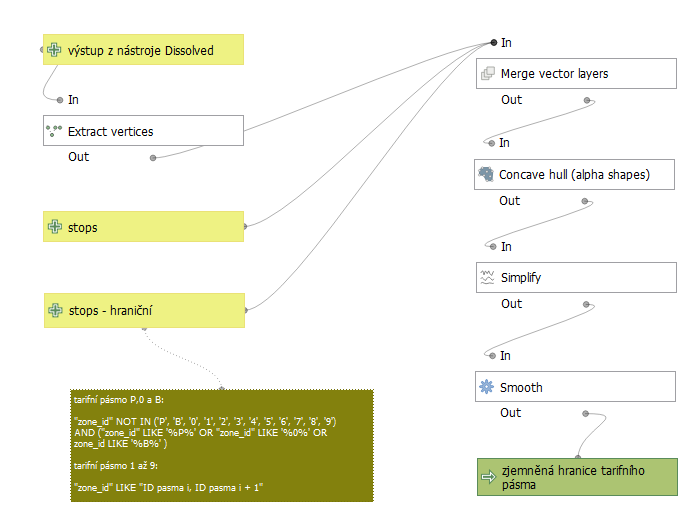
\includegraphics[width=400pt]{./pictures/postup-smooth.png}
    \caption[Postup pro zjemnění tvaru tarifních pásem]{Postup pro zjemnění tvaru tarifních pásem}
	\label{fig:postup-smooth}              
\end{figure}

\subsection{Hraniční tarifní pásma}
\label{hranice}

Jedním z největších problémů diplomové práce bylo se vypořádat s hraničním zastávkami.
V dosavadním postupu nebyl jejich problém efektivně vyřešen kvůli~kon\-kávní obálce,
která nezvládala spojovat určité body, které byly požadovány.

Naskytla se tedy myšlenka upravit algoritmus nástroje \textit{Concave hull (alpha sha\-pes)},
který je veřejně publikován ve službě GitHub jako ostatně celý zdrojový kód systému QGIS, k obrazu
svému, aby hraniční zastávky propojoval. 

Zdrojový kód nástroje byl napsán Piotrem Pociaskem v květnu 2014. Skládá se mimo jiné z nástroje
\textit{Delaunay triangulation}, který využívá pro tvorbu Delaunay triangulaci viz kapitola \ref{triangulace},
nástroje \textit{Dissolve}, nástroje \textit{Delete holes} a algoritmu alpha shapes.

\begin{figure}[H] \centering
    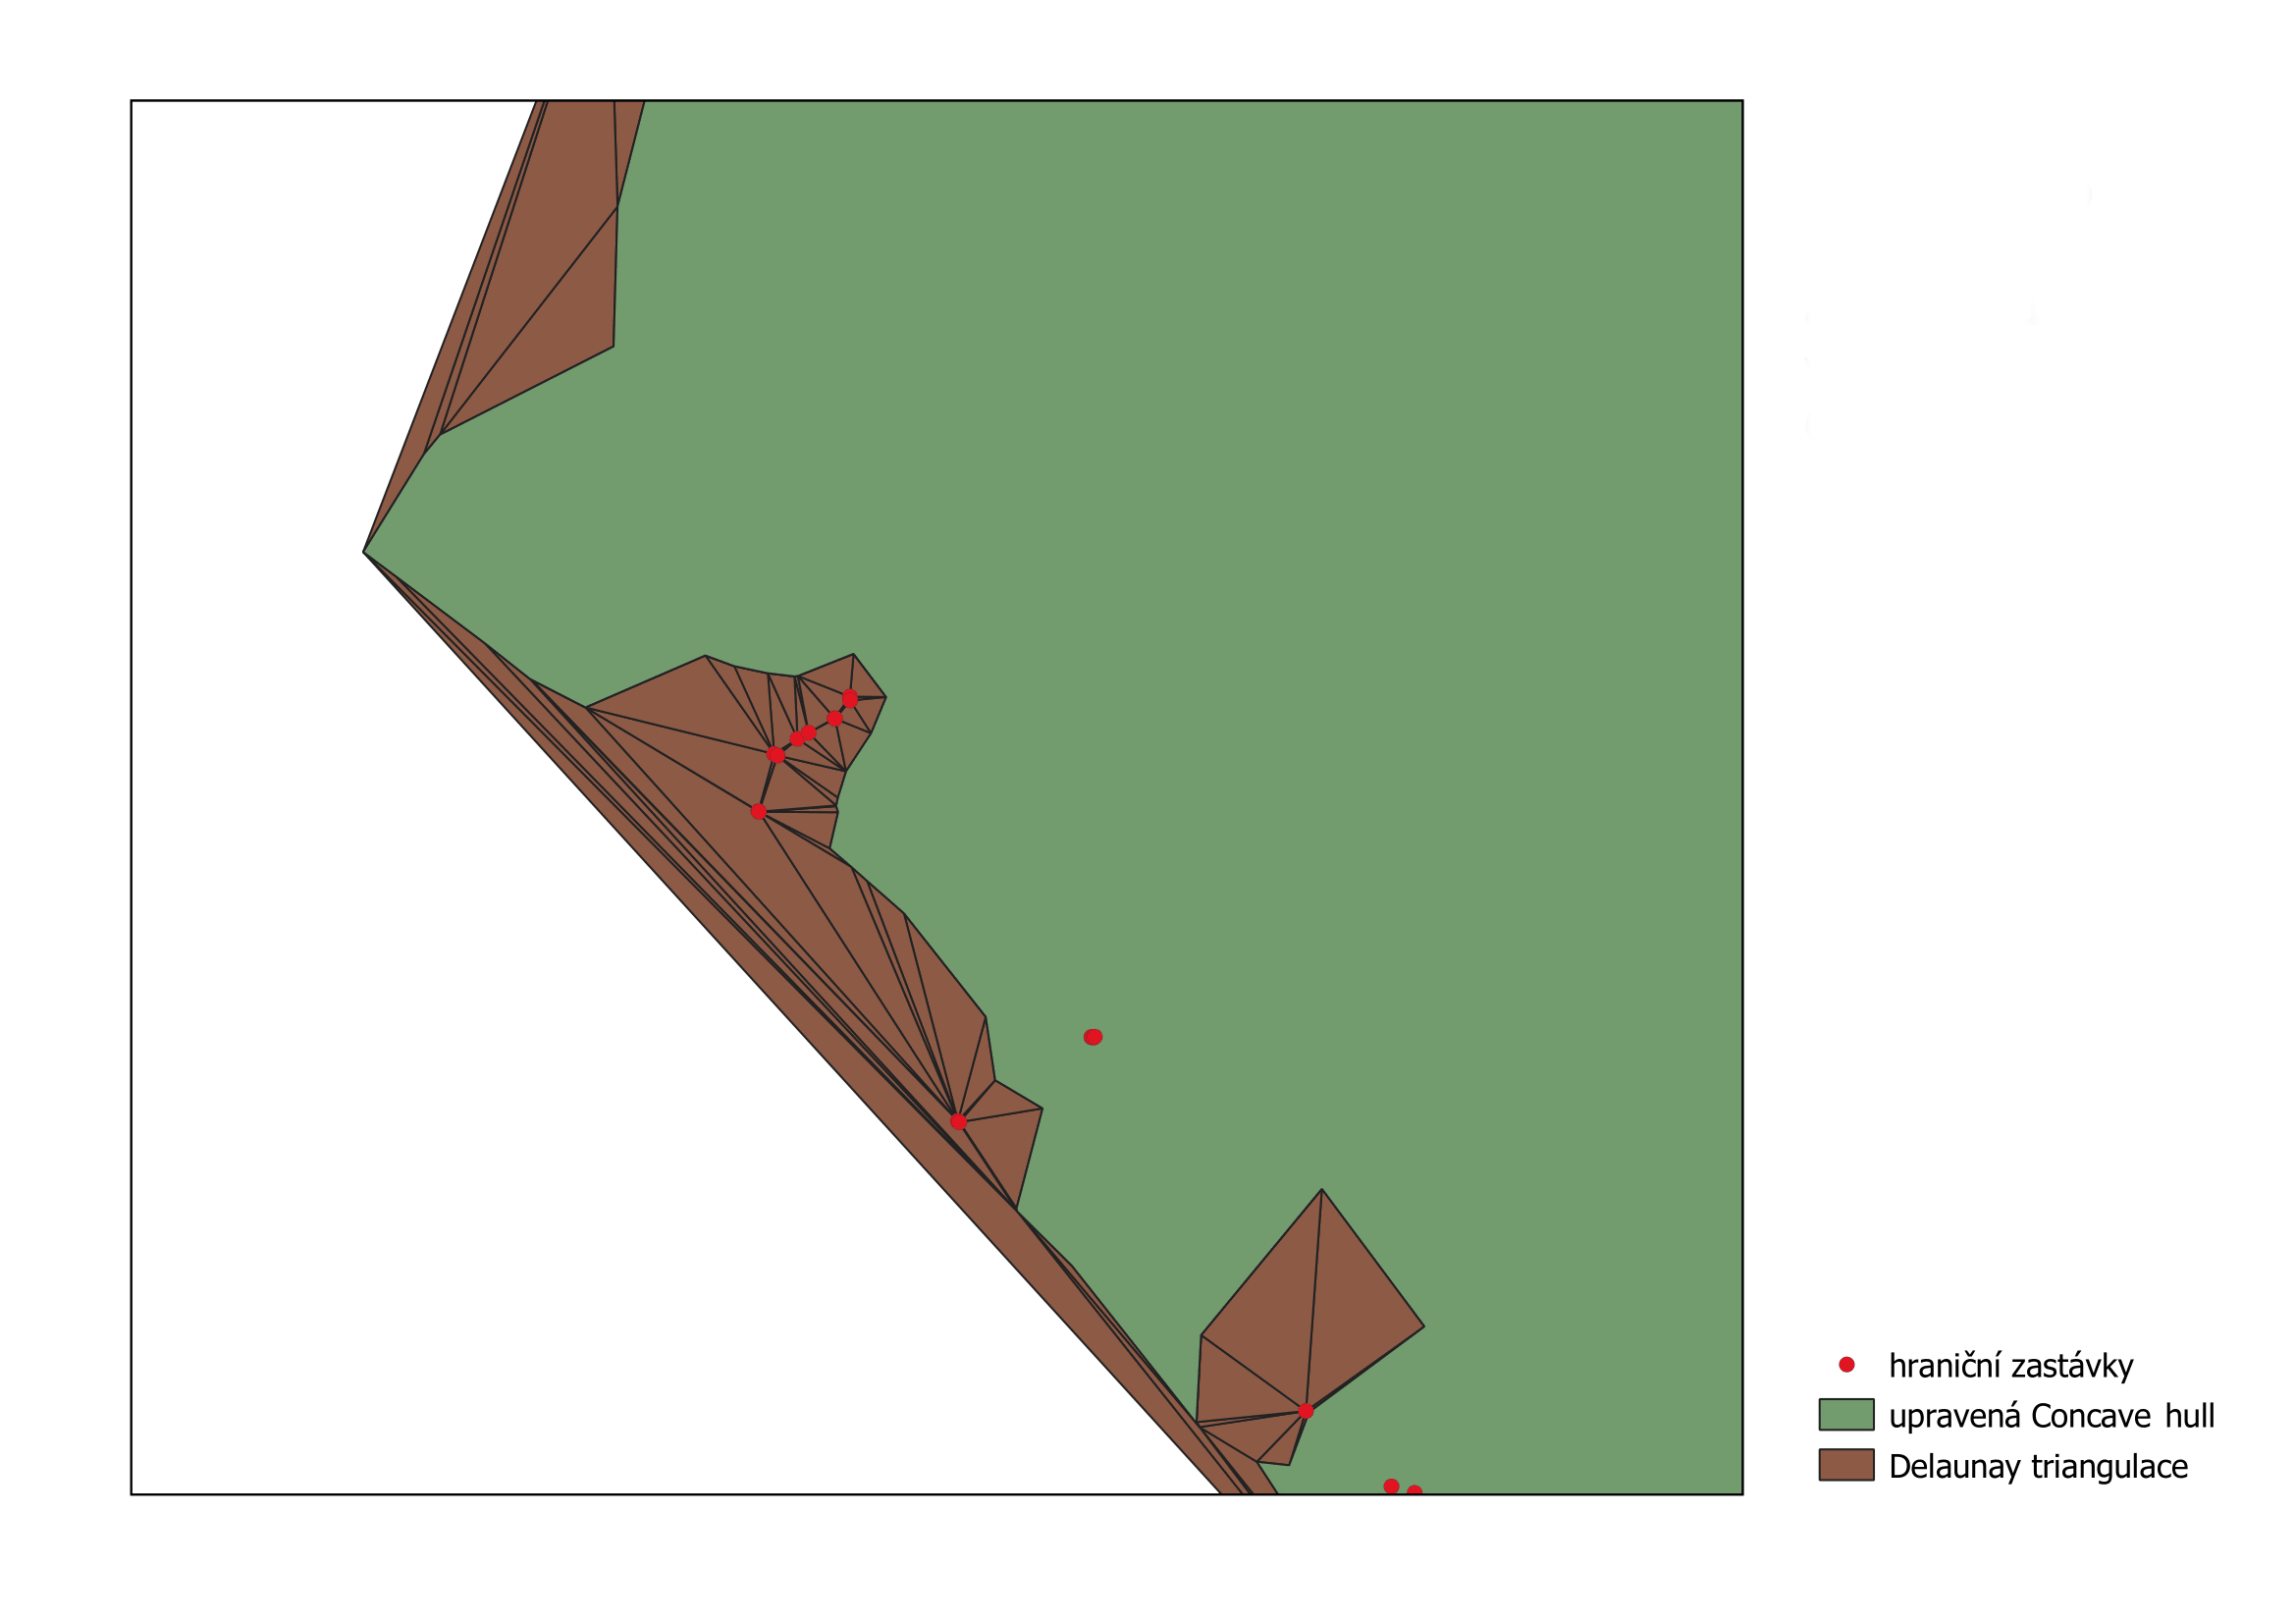
\includegraphics[width=400pt]{./pictures/concave_hull_upravena.png}
    \caption[Ukázka upravené nástroje Concave hull (alpha shapes)]{Ukázka upravené nástroje Concave hull (alpha shapes)}
	\label{fig:concave_hull_upravena}              
\end{figure}

Tento algoritmus maže ty trojúhelníky z Delaunay triangulace, které mají nejdelší stranu menší jak alpha (volitelný
parametr nástroje \textit{Concave hull (alpha sha\-pes)} násobek maximálního obvodu trojúhelníku.
K těmto trojúhelníkům byly přidá\-ny i~ty~trojúhelníky, které mají vrchol společný s jakýmkoliv hraničním bodem.

Výsledek byl oproti očekávání. Místo propojení hraničních zastávek s konkávní obálkou tam vznikly mezery, 
které se bohužel nedaly dál použit a tento postup byl zavržen.

Od pracovníků z organizace ROPID mi byl navrhnut postup, jak tento problém alespoň částečně vyřešit. Pro hraniční zastávky se stejnou hodnotou \textit{zone\_id}, 
které~leží ve své vzájemné blízkosti, vytvořit vlastní tarifní pásmo. Takový postup byl mnohem lépe uchopitelnější, než ten předchozí uvedený, který nebyl povedený.

Uložená vektorová vrstva hraničních zastávek z kapitoly \ref{vyhlazeni} byla s vektorovou vrstvou Voronoi polygonů
použita s pomocí nástroje \textit{Select by location}. Z vektorové vrstvy Voronoi polygonů byly vybrány právě ty polygony,
které se svým umístěním protínaly s hraničními zastávkami. To bylo provedeno zvlášť pro každé zastávky na~hranici tarifních pásem.

Poté byly nástrojem \textit{Dissolve} Voronoi polygony seskupeny do jednoho polygonu a jedné geometrie. Vstupem tohoto nástroje
tedy vybrané Voronoi polygony pomocí nástroje \textit{Select by location} a výstupem byla vektorová vrstva seskupených polygonů.

Toto seskupení bylo následně zrušeno pomocí nástroje \textit{Multipart to singleparts}, kde vstupem byla vektorová vrstva 
seskupených s jednou geometrií a výstupem vektorová vrstva s více geometriemi podle jejich počtu ve vektorové vrstvě.

Důvodem tohoto kroku byl úmysl spočítat počet zastávek, které ležely na území každého polygonu. Poté určit hranici
součtu zastávek a vymazat ty polygony, které~je nesplňují.

Pro spočítání zastávek byl použit nástroj \textit{Count points in polygon}. Vstupem byla vektorová vrstva 
rozdělených polygonů nástrojem \textit{Multipart to singleparts}
a~vektorová vrstva hraničních zastávek. Mimo jiných volitelných parametrů se v~nástroji nacházel i parametr 
Count field name, který určoval název nového pole s datovým typem celého čísla,
který přibyl na výstupu nástroje. Výchozí název tohoto paramet\-ru \textit{NUMPOINTS} byl ponechán. 
Kromě nového pole vypadala vý\-stupní vektorová vrstva stejně jako vstupní vektorová vrstva polygonů.

Poté podle atributového dotazu bylo rozhodnuto, jaké polygony z vektorové vrstvy polygonů vybrat do nové vektorové vrstvy.
Tento atributový dotaz vypadal následovně: 

\[NUMPOINTS > X\]

Hodnota čísla \textit{X} byla nastavena na 5. Byly vybrány ty polygony, ve kterých leželo více jak 5 zastávek.

Tento postup byl proveden for cyklem pro všechna tarifní pásma společně s~vyhlazením hranic polygonů,
jak je uvedeno v~kapitole \ref{vyhlazeni}. Na obrázku \ref{fig:postup-border-zones} je v~Grafickém modeláři zobrazen
přehledný postup pro hraniční tarifní pásma. 

\begin{figure}[H] \centering
    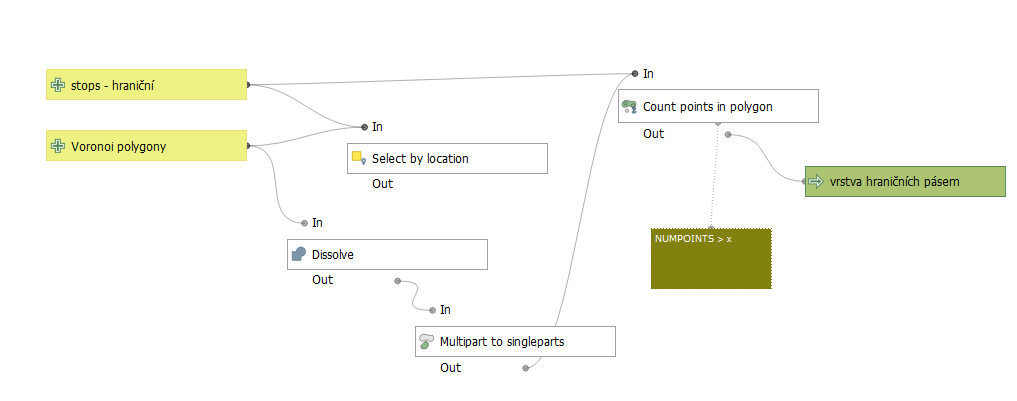
\includegraphics[width=400pt]{./pictures/postup-border-zones.png}
    \caption[Postup pro hraniční tarifní pásma]{Postup pro hraniční tarifní pásma}
	\label{fig:postup-border-zones}              
\end{figure}

\subsection{Složení tarifních pásem}
\label{seskupeni}

V dosavadním postupu byla ukládána většina polygonových vektorových vrstev do~\zk{GPKG} jako oddělené.
To bylo potřeba změnit z důvodu lepší manipulace s~výslednou vrstvou a také kvůli zmenšení velikosti \zk{GPKG}
kvůli ušetření paměti.

Vektorové vrstvy byly od sebe odečteny nástrojem \textit{Difference}, aby nebyly prolínány. 
Prvním parametrem tohoto nástroje byla vektorová vrstva, která překrývala druhou vektorovou vrstvu. 
Druhým parametrem byla vektorová vrstva, která byla překrývána. Výstupem byla odečtená vrstva.

To bylo provedeno for cyklem pro všechna tarifní pásma.

Odečtené vektorové vrstvy tarifních pásem poté byly spojeny do jedné vektorové vrstvy pomocí 
nástroje \textit{Merge vector layers}. Díky tomuto nástroji byly spojeny i~hraniční pásma zatím odděleně od tarifních pásem.

Výsledek spojení avšak obsahoval více menších polygonů se stejnými hodnotami \textit{zone\_id}.
Takové polygony bylo potřeba spojit do jednoho vícedílného polygonu pro~každou hodnotu \textit{zone\_id}.
To bylo provedeno pomocí nástroje \textit{Collect geometries}. Vstupem do tohoto nástroje byla vektorová vrstva z 
nástroje \textit{Merge vector layers} a pole, podle které se to mělo spojit, bylo nastaveno na \textit{zone\_id}.
Výstupem byla vektorová vrstva vícedílných polygonů. Tento postup byl proveden i pro hraniční pásma.

Poté zbývalo spojit vektorovou vrstvu tarifních pásem a vektorovou vrstvu hra\-ničních pásem. Kvůli vyhnutí se 
překrývání vektorových vrstev byl nejdříve použit nástroj \textit{Difference} a následně nástroj  \textit{Merge vector layers}.

Výsledkem byla jedna vektorová vrstva obsahující polygony tarifních i hraničních pásem. Na následujícím obrázku
je přehledně zobrazen postup složení v Grafickém modeláři.

\begin{figure}[H] \centering
    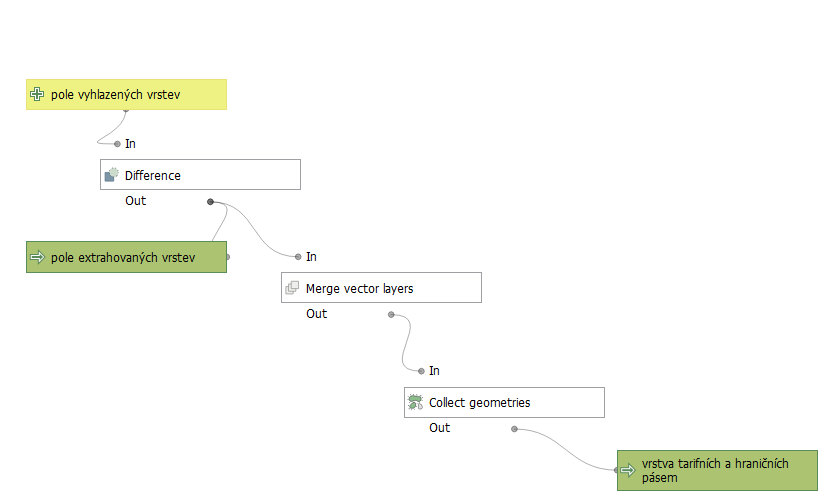
\includegraphics[width=350pt]{./pictures/postup-collecting.png}
    \caption[Postup pro složení vektorových vrstev tarifních pásem]{Postup pro složení vektorových vrstev tarifních pásem}
	\label{fig:postup-collecting}              
\end{figure}

\subsection{Symbologie tarifních pásem}
\label{symbologie}

Pro lepší vizuální vzhled výsledných tarifních pásem byla na konec procesu pluginu přidána funkce
pro obarvování pásem. To bylo provedeno díky instanci třídy \textit{QgsSymbol} a jejím metodám 
\textit{defaultSymbol} a \textit{setColor} a taktéž díky instancím tříd\textit{QgsRendererCategory}
a \textit{QgsCategorizedSymbolRenderer}.

\begin{figure}[H] \centering
    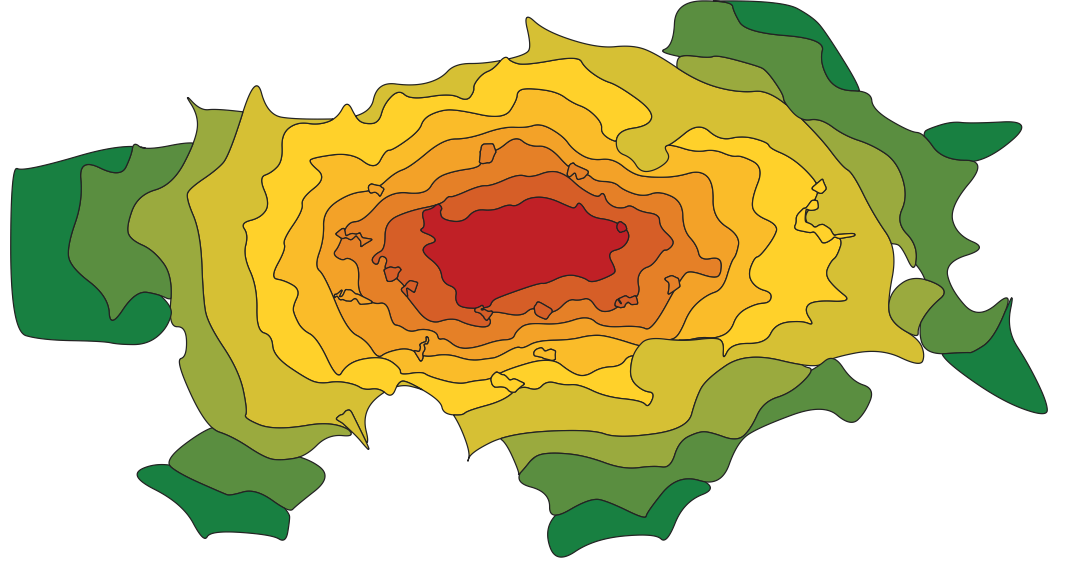
\includegraphics[width=400pt]{./pictures/vysledek2.png}
    \caption[Výsledný tvar tarifních pásem]{Výsledný tvar tarifních pásem}
	\label{fig:vysledek}              
\end{figure}

Barvy, kterými jsou výsledná tarifní pásma obarvena a které jsou zobrazeny na obrázku \ref{fig:vysledek}, byly převzaty
ze schématu tarifních pásem Pražské integrované dopravy (viz \ref{fig:pasma-schema}).  

Obrázek výsledného tvaru tarifních pásem byl vytvořen za pomocí PID\_GTFS datasetu publikováný 8. září 2020 na portálu \textit{Opendata
hlavního města Prahy}. Ve~stejný den byly zvěřejněny na stejném portálu i referenční tarifní pásma.
Avšak když byl porovnán výsledek tarifních pásem z PID\_GTFS datasetu a referenční tarifní pásma, tak
se navzájem příliš nepodobaly. Nejspíš to bylo tím, že při tvorbě referenčních tarifních pásem byly použity jiné zastávky,
než které byly publikovány s datasetem na portálu \textit{Opendata hlavního města Prahy}.
